
    The previous chapter introduced a computational idiom --
    Complex Reduction and Histogram Computations (CReHCs) -- and showed how the
    Idiom Detection Language (IDL) enables its discovery and automatic
    parallelisation.
    This chapter takes a broader view of automatic idiom detection that also
    includes common sparse and dense linear algebra computations and stencil
    codes.
    Instead of implementing bespoke parallelisation passes, the chapter
    follows the vision laid out in the introduction, using the detection results
    to translate relevant program parts into stronger models.
    Existing tools are then used to leverage the implied domain knowledge.

    The goal of this chapter is to take abstract algorithmic concepts, which are
    conventionally explored outside the context of compiler analysis --
    computational idioms -- and to formalize them as IDL specifications,
    enabling detection and manipulation in optimising compilers.
    Heterogeneous acceleration will serve as the motivation for this effort.
    As many scientific codes are structured around idiomatic performance
    bottlenecks, efforts that focus on computational idioms can greatly
    improve performance, especially with accelerators that were designed
    with similar computations in mind.
    The focus is therefore on calculations that are well supported by
    accelerators and their software ecosystems: linear algebra,
    stencil codes and CReHCs.

    The IDL specifications are used to build a prototype compiler that
    automatically detects the idioms and uses them to circumvent the code
    generator with libraries and domain specific languages:
    BLAS implementations, cuSPARSE, clSPARSE, Halide and Lift.
    The funcionality is directly accessible in a modified version of the widely
    used Clang C/C++ compilers.
    The evaluation can therefore be performed on the well established benchmark
    suites NAS and Parboil, where 60 idiom instances are detected.
    In those cases where idioms are a significant part of the sequential
    execution time, the generated heterogeneous code achieves 1.26$\times$ to
    over 20$\times$ speedup on integrated and external GPUs.

\section{Introduction}

    Heterogeneous accelerators provide the potential for superior performance.
    However, realising this potential in practice is difficult and requires
    significant programmer effort.
    Programs have to be partially rewritten to target heterogeneous systems,
    using a diverse range of broad and narrow interfaces.
    General-purpose languages such as OpenCL \citep{nvidia11guide} provide
    some portability across heterogeneous devices, but the achieved performance
    often disappoints \citep{lee09openmp}.
    Despite the functional portability, rewrites are required in practice to
    achieve competitive performance.
    Optimised numerical libraries provide more reliable performance, but they
    are more specialised and often provided by hardware vendors without
    portability in mind \citep{clblas,cublas,cusparse,clsparse}.
    More narrow domain-specific languages (DSLs) have been proposed by
    \citet{Ragan-Kelley2013Halide,Franchetti09OL,Rompf:2012:LMS:2184319.2184345}
    among others in attempts to deliver both portability and performance.
    However, this class is quickly evolving, and with most of these DSLs being
    academic projects, the adoption and long term support remain unclear.

    Hardware is becoming increasingly heterogeneous, most recently with the
    development of deep neural network accelerators such as the Google TPU
    \citep{jouppi2017datacenter}.
    This means that library or DSL based programming is likely to become far
    more common.
    The problems with this trend that arise due to the aforementioned tradeoffs
    are evident:
    Firstly, application developers have to learn multiple specialised DSLs and
    vendor-specific libraries if they want good performance.
    Secondly, they will have to rewrite their existing applications to use them.
    Thirdly, this ties code into an ecosystem with unclear future support
    that might soon become obsolete.
    This situation is a severe impediment to the wide-spread efficient
    exploitation of heterogeneous hardware.

    The ideal would be a compiler that automatically maps existing code to
    heterogeneous hardware, with full performance and requiring no directions
    from the application programmer.
    While this is unrealistic in general, the chapter presents a system that
    approximates such a general-purpose system by utilising know-how that is
    already available and encapsulated in the existing backend interfaces.
    Instead of implementing code generation for each heterogeneous
    accelerator, the system maps user code to heterogeneous hardware using the
    existing libraries and domain-specific languages, effectively outsourcing
    the code generation to hardware and domain specialists.

    The approach is based on detecting specific {\em computational idioms} in
    application code that correspond to the functionality of existing interfaces
    -- libraries and DSLs -- for heterogeneous acceleration.
    In addition to the Complex Reduction and Histogram Computations (CReHCs)
    introduced in \Cref{chapter:reductions}, the focus is on
    sparse and dense linear algebra, as well as stencils.
    The covered idioms are a reflection of both the most relevant program
    bottlenecks and the available interfaces.
    Some computational idioms are more widely supported than others, potentially
    pointing to gaps in the accelerator landscape, but some backend was
    available for each of them.
    The Idiom Detection language (IDL) then enabled the automatic detection of
    idioms.

    Once detected, the idioms are mechanically translated into the appropriate
    DSL or replaced with a library call.
    This optimised code, or the pre-built optimised library, is then linked into
    the original program.
    As backends, the libraries cuSparse, clSparse, cuBLAS, clBLAS for
    sparse and dense linear algebra and the DSLs Halide
    \cite{Ragan-Kelley2013Halide} and Lift \cite{SteuwerRD17} were used in the
    evaluation.
    The Lift language is a data-parallel functional language that supports
    generalised reductions as well as stencils and linear algebra.
    The wide range of backends allows the freedom to target many APIs per idiom
    and pick the implementation that best suits the target platform.

    New computational idioms can be easily added thanks to the flexibility of IDL.
    This also provides a powerful means of determining whether a proposed
    heterogeneous interface matches existing code, without touching the core
    compiler.
    The idioms addressed in this paper can be expressed in less than 500 lines
    of IDL code.
    The approach is also highly robust, has been applied to the entire NPB
    and Parboil benchmark suites and was evaluated on three platforms.

    The chapter presents a novel approach that:
    \begin{itemize}
    \item Proposes the Idiom Detection Language (IDL) for detecting idiomatic
          code sections that can be accelerated by domain-specific backends.
    \item Implements several common computational idioms in IDL to automatically
          discover opportunities for accelerator exploitation.
    \item Efficiently translates and maps the detected idioms to APIs for
          heterogeneous systems.
    \end{itemize}

    The work most similar in approach discovers stencil computations and maps to
    the Halide DSL for acceleration.
    The Helium tool \citep{Mendis2015Helium} recovers stencils from
    image-processing binaries.
    This requires large scale dynamic analysis of binary traces and replacing
    them with Halide calls. 
    This is significantly extended by \citet{Kamil2016Verified}, detecting
    stencils in Fortran code.
    The focus of that work is on inferring post invariants based on syntax
    guided synthesis in translation to Halide.
    However, it uses a narrow approach to selecting code snippets and relies on
    well-structured Fortran with occasional user annotations.
    The IDL approach is distinct in its use of an external programming language
    for the flexibility of describing arbitrary idioms.
    This allows an unbounded set of idioms to be considered and is not
    restricted to stencils. 

    To summarise, this chapter presents an automatic approach that discovers
    idioms in legacy code and maps them to heterogeneous platforms via libraries
    and DSLs.
    The tool was applied to 21 C/C++ programs from the NPB and Parboil benchmark
    suites, where it detected more reductions, stencils, matrix multiplications
    and sparse matrix-vector computations than existing schemes.
    For the programs where idioms dominate execution time, accelerator code
    was generated and evaluated on 3 platforms: a multi-core CPU, an integrated
    APU, and an external GPU.
    Overall, 60 idioms were detected, and they dominated execution time in
    10 programs.
    Speedup results for the accelerated code ranged from 1.26$\times$ to over
    20$\times$.

\section{Overview}

    The approach is automatic and has been implemented inside the LLVM compiler
    infrastructure.
    It takes arbitrary sequential C/C++ programs as input.
    Using the Clang compiler, the input source code is compiled into a Static
    Single Assignment (SSA) intermediate representation (LLVM IR).
    In this representation, the specified idioms are identified and replaced
    with calls to specific APIs.
    Finally, the code generated by the LLVM compiler and the output of the idiom
    specific code generators/libraries are linked together into a binary,
    producing an optimised program.
    LLVM was chosen as it is the best supported SSA-based compiler;
    the methodology could easily be transferred to other infrastructures such as
    GCC.

\subsection{Compiler Flow}

    The structure of the approach is described in more detail in
    \Cref{fig:methodology}.
    The compiler takes two programs as inputs: the first is the source code of
    the user program, the second describes the computational idioms that are to
    be detected specified in IDL.
    The same idioms, of course, can be detected across many user programs.
    Therefore, the IDL program does not have to change from one run to the next.

\begin{figure}[p]
    \centering
    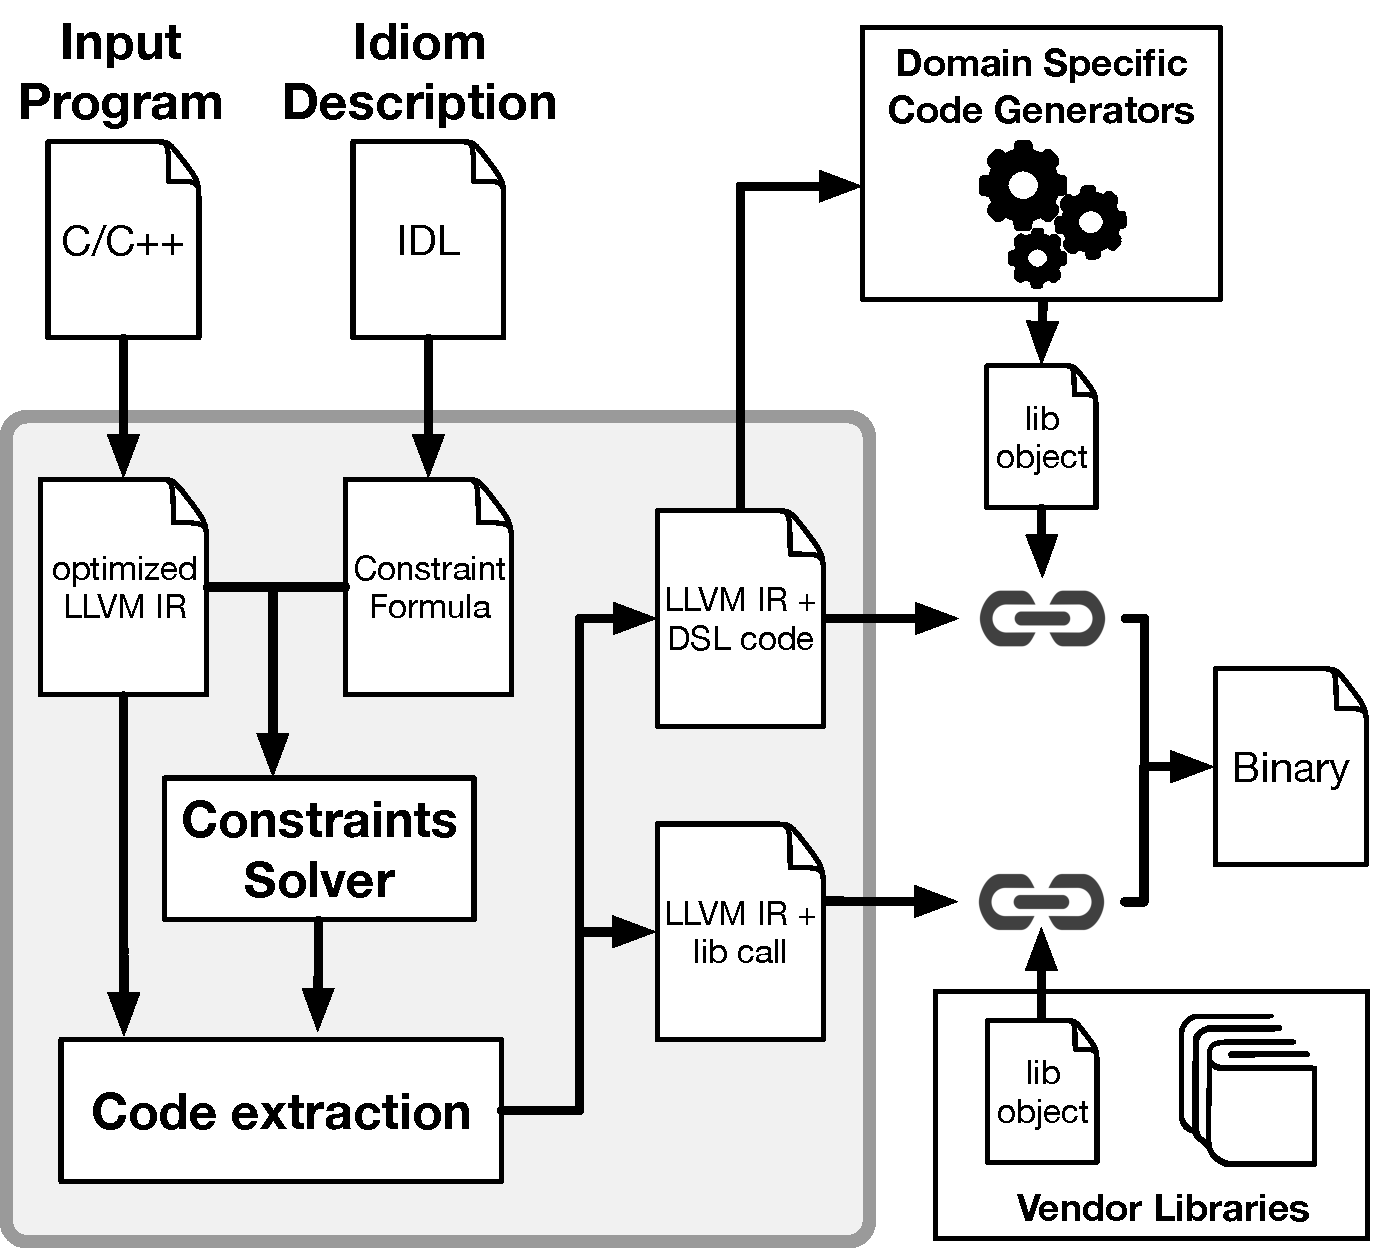
\includegraphics[width=\linewidth]{figures/compiler_flow.pdf}
    \caption{Workflow of the IDL acceleration system:
             The IDL solver extracts idiomatic loops in the optimised LLVM IR
             of user programs.
             These loops are extracted and replaced with shim function calls.
             Domain-specific code generators implement the calls as library
             objects, or they are taken directly from pre-generated vendor
             libraries for idioms not containing kernel functions.}
    \label{fig:methodology}
\end{figure}

    The source code of the user program is compiled into optimised LLVM IR code,
    and the idiom description is parsed and represented internally as a C++
    object, as previously described in \Cref{chapter:theory},
    \Cref{subsec:impl}.
    The C++ representation of the constraints and the LLVM IR code
    are then passed as inputs to the backtracking solver, which detects all
    cases where the idioms can be found in the LLVR IR.

    The recognised idioms and the LLVM IR code are then passed on to the
    transformation phase of the system.
    The sections of code corresponding to computational idioms are extracted
    and then reformulated for the appropriate heterogeneous backends.
    For libraries, this means replacing the code covered by the idiom with a
    library call. 

    For DSL interfaces, the process is a little more involved.
    The user code captured by idioms is extracted and replaced with functions
    calls to shim interfaces.
    The extracted code features are translated into the appropriate DSL and
    passed on to the external DSL compiler, which optimises it and generates a
    library object that implements the required function interfaces.
    The translation to DSL mainly involves representing the kernel functions.
    Idioms without kernel functions correspond to fixed DSL programs and
    require no additional work.
    The generated code is then linked with the object code from the main program.

    Determining the best heterogeneous APIs to use for a given platform and the
    best idioms to exploit will become an essential consideration as the number
    of idioms and APIs grows.
    Currently, for this chapter, all applicable libraries and DSLs were
    evaluated, and the best-performing versions selected after profiling.

\subsection{Accelerating Sparse Linear Algebra}

    Sparse linear algebra is central to many scientific codes and increasingly
    important as a basis for graph algorithms and data analytics
    \cite{Kepner2015GraphsMA}, but they contain indirect data access that limits
    compiler optimisation.
    Instead, programmers rely on library implementations that are hand optimised
    and utilise accelerator hardware.
    This reliance on libraries comes at a cost, however, as it ties programs
    into vendor-specific software ecosystems and results in non-portable code.
    The IDL approach offers an alternative by recognising sparse linear algebra
    operations in compiler intermediate representation and then incorporating
    domain-specific backends without source code changes.

    The code at the top of \Cref{fig:spmvexample1} is the performance
    bottleneck of the ``Conjugate Gradient'' benchmark program in the NAS
    Parallel Benchmarks, with the corresponding LLVM~IR code underneath.
    This bottleneck loop implements a standard operation from sparse linear
    algebra, namely the multiplication of a sparse matrix in
    Compressed Sparse Row (CSR) format with a dense vector.
    This computation is supported on accelerator hardware, using well-optimised
    libraries such as cuSPARSE and clSPARSE.
    However, compilers are unable to recognise and accelerate the computation
    automatically.

    The structure of this sparse linear algebra computation has several features
    that make it unsuitable for most established compiler optimisations:
    Firstly, the iteration domain of the nested loop is memory dependent
    (line 3), and secondly, there is indirect memory access (line~4).
    This makes the iteration domain of the loop nest as a whole non-polyhedral
    and the access structure to memory non-affine.
    Under these conditions, simple data dependence models, but also
    sophisticated analysis based on the polyhedral model, fail.

    IDL can express this sparse idiom, as derived in \Cref{sec:idioms},
    \Cref{csr_lilacwhat_fig}.
    The ``Conjugate Gradient'' LLVM IR code, together with the ``SPMV-CSR''
    IDL specification, are input to the constraint solver, which outputs a
    constraint solution, as shown in \Cref{fig:spmvexample2}.
    In the solution, different values for the LLVM IR have been assigned to all
    IDL variables in the ``SPMV-CSR'' specification.

    \Cref{fig:spmvexample3} shows how this solution is used to generate a
    call to a cuSPARSE procedure.
    The individual solution variables are inserted into the {\tt cusparseDcsrmv}
    code template as function arguments. 
    The original code is then cut out and replaced with this function call.
    In practice, this involves a shim function that manages the device context
    and memory transfers from and to the GPU.
    Finally, the cuSPARSE library is linked with the object code produced by the
    Clang compiler, resulting in a speedup of $17\times$ on a GPU as described
    in more detail in\Cref{sec:idiomresults}.

    Central to this approach is the ability to detect computational idioms
    reliably.
    The next section derives in detail the formulation of linear algebra -- both
    sparse and dense -- and stencils in the Idiom Detection Language.

\begin{figure}[p]
    \begin{lstlisting}[language=MyCpp, basicstyle=\linespread{0.75}\small\ttfamily]
for (j = 0; j < ([{\bf m}]); j++) {
  d = 0.0;
  for (k = ([{\bf rowstr }])[j]; k < ([{\bf rowstr}])[j+1]; k++)
    d = d + ([{\bf a}])[k]*([{\bf z}])[([{\bf colidx}])[k]];
  ([{\bf r}])[j] = d; }
\end{lstlisting}
\vspace{-4.4mm}
\begin{lstlisting}[language={LLVM}, basicstyle=\linespread{0.75}\tiny\ttfamily,
                   label={fig:spmvexample1}, caption={Sparse linear algebra in C and LLVM IR}]
; <label>:2:
  %j = phi i64 [ %j_next, %12 ], [ 0, %1 ]
  %j_cond = icmp slt i64 %j, ([{\bf \%m}])
  br i1 %j_cond, label %3, label %13([\vspace{1mm}])
; <label>:3:
%4 = getelementptr i32, i32* ([{\bf \%rowstr}]), i64 %j
  %5 = load i32, i32* %4
  %j_next = add nuw nsw i64 %j, 1
  %6 = getelementptr i32, i32* ([{\bf \%rowstr}]), i64 %j_next
  %7 = load i32, i32* %6
  %k_begin = sext i32 %5 to i64
  %k_end = sext i32 %7 to i64
  br label %8([\vspace{1mm}])
; <label>:8:
  %k = phi i64 [ %k_next, %9 ], [ %k_begin, %dnext ]
  %d = phi double [ 0.0, %3 ], [ %d_next, %9 ]
  %k_cond = icmp slt i64 %iv, %k_end
  br i1 %k_cond, label %9, label %12([\vspace{1mm}])
; <label>:9:
  %a_addr = getelementptr double, double* ([{\bf \%a}]), i64 %k
  %a_load = load double, double* %a_addr
  %cix_addr = getelementptr i32, i32* ([{\bf \%colidx}]), i64 %k
  %cix_load = load i32, i32* %cix_addr
  %10 = sext i32 %cix_load to i64
  %z_addr = getelementptr double, double* ([{\bf \%z}]), i64 %10
  %z_load = load double, double* %z_addr
  %11 = fmul double %a_load, %z_load
  %d_next = fadd double %d, %11
  %k_next = add nsw i64 %k, 1
  br label %8([\vspace{1mm}])
; <label>:12:
  %r_addr = getelementptr double, double* ([{\bf \%r}]), i64 %j
  store double %d, double* %r_addr
  br label %2
\end{lstlisting}
\vspace{-0.287cm}
%\end{figure}

\centering
\vspace{0.0em}
{\centering
\begin{minipage}{0.05\linewidth}
\vspace{0pt}
\centering
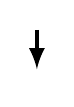
\begin{tikzpicture}[ultra thick]
 \draw [black,   -latex      ] (0,0.5) -- (0,0) node [] {};
\end{tikzpicture}
\end{minipage}
\begin{minipage}{\linewidth}
% \vspace{-5pt}
\centering
\textbf{Idiom detection with IDL program in \Cref{fig:spmv}}
\end{minipage}
\begin{minipage}{0.05\linewidth}
\vspace{0pt}
\centering
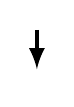
\begin{tikzpicture}[ultra thick]
 \draw [black,   -latex      ] (0,0.5) -- (0,0) node [] {};
\end{tikzpicture}
\end{minipage}
}

%\begin{figure}
{\centering
\footnotesize 
\begin{tabular}{l|l}
\textbf{Variable Name} & \textbf{Assigned IR Value}\\
\hline
iterator                    & \texttt{\%j}\\
inner.iter\_begin           & \texttt{\%k\_begin}\\
inner.iter\_end             & \texttt{\%k\_end}\\
inner.iterator              & \texttt{\%k}\\
idx\_read.value             & \texttt{\%cix\_load}\\
indir\_read.value           & \texttt{\%a\_load}\\
seq\_read.value             & \texttt{\%z}\\
\end{tabular}
\hspace{0.5cm}
\begin{tabular}{l|l}
\textbf{Variable Name} & \textbf{Assigned IR Value}\\
\hline
output.address              & \texttt{\%r\_addr}\\
iter\_begin                 & \texttt{0}\\
iter\_end                   & \texttt{\%\bf m}\\
idx\_read.base\_pointer     & \texttt{\%\bf colidx}\\
seq\_read.base\_pointer     & \texttt{\%\bf a}\\
indir\_read.base\_pointer   & \texttt{\%\bf z}\\
\dots                       & \dots\vspace{-0.5mm}\\
\end{tabular}

}

\caption{Constraint solution for sparse mv}
\label{fig:spmvexample2}
%\end{figure}

\centering
\vspace{0.0em}
{\centering
\begin{minipage}{0.05\linewidth}
\vspace{0pt}
\centering
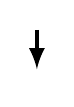
\begin{tikzpicture}[ultra thick]
 \draw [black,   -latex      ] (0,0.5) -- (0,0) node [] {};
\end{tikzpicture}
\end{minipage}
\begin{minipage}{\linewidth}
% \vspace{-5pt}
\centering
\textbf{Code generation: insert arguments, replace code}
\end{minipage}
\begin{minipage}{0.05\linewidth}
\vspace{0pt}
\centering
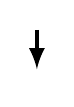
\begin{tikzpicture}[ultra thick]
 \draw [black,   -latex      ] (0,0.5) -- (0,0) node [] {};
\end{tikzpicture}
\end{minipage}
}


%\begin{figure}
\begin{lstlisting}[language=C, basicstyle=\linespread{0.75}\small\ttfamily,
                   label={fig:spmvexample3}, caption={Generated function call to cuSPARSE}]
cusparseDcsrmv(context,
    CUSPARSE_OPERATION_NON_TRANSPOSE, ([{\bf m}]), n,
    ([{\bf rowstr}])[([{\bf m}])+1]-([{\bf rowstr}])[0], &gpu_1, descr, gpu_([{\bf a}]),
    gpu_([{\bf rowstr}]), gpu_([{\bf colidx}]), gpu_([{\bf z}]), &gpu_0, gpu_([{\bf r}]));
\end{lstlisting}
\vspace{-0.287cm}
\end{figure}

\section{Specification of Idioms in IDL}
\label{sec:idioms}

    The specification of computational idioms in IDL requires careful
    handling of the arising complexity, using the modularity functionality that
    IDL provides.
    Control flow constructs, memory access patterns as well as basic data flow
    patterns are specified independently and then combined in order to define
    the complete constraint specifications.
    This section extends upon the previously defined building blocks from
    \Cref{chapter:candl,chapter:reductions}.

\subsection{Sparse Linear Algebra}

    The most frequently used performance-critical sparse linear algebra routines
    are variations on the multiplication of a sparse matrix with a dense vector
    (SPMV).
    Crucial for these sparse linear algebra routines is capturing the many
    different memory access patterns.
    On the other hand, the control flow is very rigid.

    \Cref{spmvbase} shows the basic skeleton of the SPMV idiom:
    There are two for-loops, the {\tt outer\_loop} and the {\tt inner\_loop}.
    Naturally, {\tt outer\_loop} has to contain {\tt inner\_loop} fully
    (lines 4--7).
    The outer loop is a standard for-loop (line 2), while the inner loop is a
    for-loop that also contains a generalised dot product (line 3).
    Specifically, the {\tt DotProductFor} specification requires that the
    loop contains a scalar reduction variable that in every iteration is
    incremented by the result of a floating-point multiplication of two values
    {\tt src1} and {\tt src2}.
    This skeleton is completed depending on the sparse matrix format, defining
    the specific computations and data flow that yields {\tt src1} and
    {\tt src2}.

\begin{figure}[p]
\lstset {
 basicstyle=\linespread{1.069}\small\ttfamily
}
\begin{lstlisting}[language=IDL, label={spmvbase}, caption=
   {Skeleton of the sparse matrix-vector product (SPMV) constraint
    specification in IDL: The precise sparse access patterns are specific to
    chosen storage formats for sparse matrices.}]
Constraint SPMV
( inherits For at {outer_loop} and
  inherits DotProductFor at {inner_loop} and
  {outer_loop.begin} strictly
      control flow dominates {inner_loop.begin} and
  {outer_loop.end} strictly
      control flow post dominates {inner_loop.end} and
([\dots])
\end{lstlisting}
\end{figure}

\begin{figure}[p]
\hfill
\begin{minipage}[b]{0.3\linewidth}
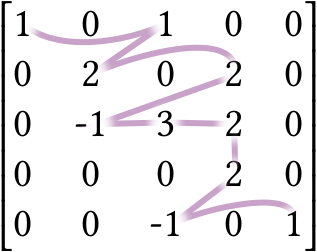
\includegraphics[width=0.95\linewidth]{figures/csrorder.png}
\end{minipage}
\hfill
\begin{minipage}[b]{0.5\linewidth}
\begin{align*}
\text{\bf val} =& \begin{bmatrix}
1\ \ 1\ \ 2\ \ 2\ \ \text{-}1\ \ 3\ \ 2\ \ 2\ \ \text{-}1\ \ 1\\
\end{bmatrix}\\[4mm]
\text{\bf col\_ind} =& \begin{bmatrix}
0\ \ 2\ \ 1\ \ 3\ \ 1\ \ 2\ \ 3\ \ 3\ \ 2\ \ 4\\
\end{bmatrix}\\[4mm]
\text{\bf row\_ptr} =& \begin{bmatrix}
0\ \ 2\ \ 4\ \ 7\ \ 8\ \ 10\\
\end{bmatrix}
\end{align*}
\end{minipage}
\hfill

\vspace{0.8em}
\hrule
\vspace{0.3em}

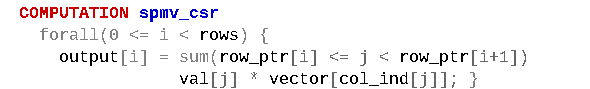
\includegraphics[width=\linewidth]{figures/spmvcsrwhat.pdf}
\vspace{-1.5em}
\lstset {
 basicstyle=\linespread{1.069}\small\ttfamily
}
\begin{lstlisting}[language=IDL,firstnumber=7]
([\dots])
  inherits VectorStore
      with {outer_loop}          as {scope}
       and {outer_loop.iterator} as {input_index} at {output} and
  inherits VectorRead
      with {outer_loop}          as {scope}
       and {inner_loop.src1}     as {value}
       and {inner_loop.iterator} as {input_index} at {val} and
  inherits VectorRead
      with {outer_loop}      as {scope}
       and {inner_loop.src2} as {value}
       and {col_ind.value}   as {input_index} at {vector} and
  inherits VectorRead
      with {outer_loop}          as {scope}
       and {inner_loop.iterator} as {input_index} at {col_ind} and
  inherits ReadForLoopRanges
     with {outer_loop}          as {scope}
      and {inner_loop}          as {for}
      and {outer_loop.iterator} as {input_index} at {row_ptr})
End
\end{lstlisting}
\caption{Compressed Sparse Row in IDL:
         The top section of the figure shows the different involved arrays.
         The pseudocode in the middle row of the
         figure then directly gives a completion of \Cref{spmvbase}.
         Walking through the expressions and emitting IDL code on-by-one is
         sufficient.}
\label{csr_lilacwhat_fig}
\end{figure}

\subsubsection{Compressed Sparse Row}

    The Compressed Sparse Row (CSR) format is one of the most widely used
    formats for sparse matrices \cite{doi:10.1137/1.9780898718003}.
    An example matrix stored in CSR format is shown at the top of
    \autoref{csr_lilacwhat_fig}.
    The 5x5 matrix on the left is stored in the three separate arrays on the
    right: \textbf{val}, \textbf{col\_ind}, and \textbf{row\_ptr}.

    All non-zero entries of the matrix are stored in a flat array \textbf{val}
    in a row-by-row order.
    The \textbf{col\_ind} array stores the column position for each value.
    Finally, the \textbf{row\_ptr} array stores the beginning of each row of the
    matrix as an offset into the other two arrays.
    The number of rows in the matrix is given directly by the length of the
    \textbf{row\_ptr} array minus one.
    However, the number of columns is not explicitly stored.

    The middle row of \autoref{csr_lilacwhat_fig} shows the corresponding
    SPMV computation in pseudocode.
    Finally, the bottom of the figure shows the continuation of the {\tt SPMV}
    IDL specification for CSR matrices.
    This continuation is immediately derived by walking through the pseudocode
    expressions and emitting {\tt inherits} directives to the corresponding
    IDL subprograms.

\subsubsection{Jagged Diagonal Storage}

    For Jagged Diagonal Storage (JDS) \cite{doi:10.1137/0910073}, the rows of
    the matrix are permuted such that the number of nonzeros per row  decreases.
    The permutation is stored in a vector \textbf{perm}, the number of nonzeros
    in \textbf{nzcnt}.
    The nonzero entries are then stored in an array \textbf{val} in the
    following order:
    The first nonzero entry in each row, then the second nonzero entry in
    each row and so on.
    The array \textbf{col\_ind} stores the column for each of the values and
    \textbf{jd\_ptr} stores offsets into \textbf{val} and \textbf{col\_idx}.

    \autoref{jds_lilacwhat_fig} demonstrates this format on the example sparse
    matrix from \autoref{csr_lilacwhat_fig}, and derives the corresponding IDL
    code for the {\tt SPMV\_JDS} idiom underneath.
    Note that the sparse matrix in this example is shown after the permutation
    operation that JDS requires.

\begin{figure}[p]
\hfill
\begin{minipage}[b]{0.3\linewidth}
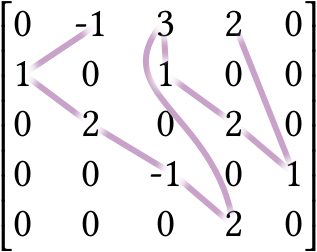
\includegraphics[width=0.9\linewidth]{figures/jdsorder.png}
\end{minipage}
\hfill
\begin{minipage}[b]{0.65\linewidth}
\footnotesize
\begin{align*}
\text{\bf perm} =& \begin{bmatrix}1\ \ 2\ \ 0\ \ 4\ \ 3\\\end{bmatrix}\\[-0.75mm]
\text{\bf val} =& \begin{bmatrix}\text{-}1\ \ 1\ \ 2\ \ \text{-}1\ \ 2\ \ 3\ \ 1\ \ 2\ \ 1\ \ 2\\\end{bmatrix}\\[-0.75mm]
\text{\bf col\_ind} =& \begin{bmatrix}1\ \ 0\ \ 1\ \ 2\ \ 3\ \ 2\ \ 2\ \ 3\ \ 4\ \ 3\\\end{bmatrix}\\[-0.75mm]
\text{\bf jd\_ptr} =& \begin{bmatrix}0\ \ 5\ \ 9\ \ 10\\\end{bmatrix}\\[-0.75mm]
\text{\bf nzcnt} =& \begin{bmatrix}3\ \ 2\ \ 2\ \ 2\ \ 1\end{bmatrix}
\end{align*}
\end{minipage}
\hfill

\vspace{0.8em}
\hrule
\vspace{0.3em}

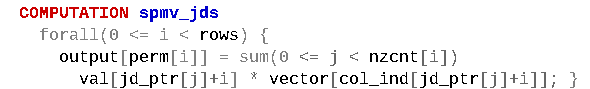
\includegraphics[width=\linewidth]{figures/spmvjdswhat.pdf}
\vspace{-1.5em}
\lstset {
 basicstyle=\linespread{1.271}\small\ttfamily
}
\begin{lstlisting}[language=IDL,firstnumber=7]
([\dots])
  inherits VectorStore
      with {outer_loop} as {scope}
       and {perm.value} as {input_index} at {output} and
  inherits VectorRead
      with {outer_loop}          as {scope}
       and {outer_loop.iterator} as {input_index} at {perm} and
  inherits VectorRead
      with {outer_loop}      as {scope}
       and {inner_loop.src1} as {value}
       and {tmp1.value}      as {input_index} at {val} and
  inherits Addition
      with {jd_ptr.value}        as {input}
       and {outer_loop.iterator} as {addend} at {tmp1} and
  inherits VectorRead
      with {outer_loop}          as {scope}
       and {inner_loop.iterator} as {input_index} at {jd_ptr} and
  inherits VectorRead
      with {outer_loop}      as {scope}
       and {inner_loop.src2} as {value}
       and {col_ind.value}   as {input_index} at {vector} and
  inherits VectorRead
      with {outer_loop} as {scope}
       and {tmp1.value} as {input_index} at {col_ind} and
  inherits ReadForLoopIterations
     with {outer_loop}          as {scope}
      and {inner_loop}          as {for}
      and {outer_loop.iterator} as {input_index} at {read_range}
\end{lstlisting}
\caption{Jagged Diagonal Storage in IDL:
         The top section of the figure shows the different involved arrays.
         The pseudocode in the middle row of the
         figure then directly gives a completion of \Cref{spmvbase}.
         Walking through the expressions and emitting IDL code on-by-one is
         sufficient.}
\label{jds_lilacwhat_fig}
\end{figure}

\subsection{Dense Linear Algebra}

    Describing dense linear algebra does not require storage format
    consideration aside from the simple {\it row-major} and {\it column-major}
    distinction.
    The generalised matrix multiplication idiom is shown in \Cref{fig:gemm}.
    The control flow is captured by three nested for loops.
    Inside these loops, the memory access is characterised by three matrix
    accesses, each with a different subset of the loop iterators.
    The corresponding \texttt{MatrixRead} and \texttt{MatrixWrite} idioms model
    generic access to matrices allowing strides, transposed matrices etc.
    The actual computation is encapsulated by the
    \texttt{DotProductForAlphaBeta} idiom, which extends the
    \texttt{DotProductFor} specification to capture the the linear combination
    with factors \texttt{alpha} and \texttt{beta} that is part of the
    generalised matrix multiplication idiom ($C\gets\alpha AB+\beta C$).

\begin{figure}[H]
\lstset {
 basicstyle = \linespread{0.865}\ttfamily
}
\begin{lstlisting}[language=IDL, label={fig:gemm}, caption=
   {IDL specification of the generalised dense matrix-vector multiplication
    (GEMM)\leftskip=0pt\rightskip=0pt}]
Constraint GEMM
( inherits ForNest(N=3) and
  inherits MatrixStore
      with {iterator[0]} as {col}
       and {iterator[1]} as {row}
       and {begin} as {begin} at {output} and
  inherits MatrixRead
      with {iterator[0]} as {col}
       and {iterator[2]} as {row}
       and {begin} as {begin} at {input1} and
  inherits MatrixRead
      with {iterator[1]} as {col}
       and {iterator[2]} as {row}
       and {begin} as {begin} at {input2} and
  inherits DotProductForAlphaBeta
      with {loop[2]}        as {loop}
       and {input1.value}   as {src1}
       and {input2.value}   as {src2}
       and {output.address} as {update_address})
End
\end{lstlisting}
\end{figure}

\subsection{Stencils}

    \Cref{fig:stencilcompute} shows the base version of the stencil idiom.
    Stencils consist of a loop nest with multi-dimensional memory access
    (lines 3--5) to store the updated cell value.
    The updated value is computed by a kernel function (lines 12--13) using
    several values that are constrained by \texttt{StencilRead} (lines 6--10),
    which specifies multi-dimensional array access with only constant offsets in
    all dimensions.

\begin{figure}[t]
\begin{lstlisting}[language=IDL, label={fig:stencilcompute}, caption=
   {IDL specification of a basic stencil computation}]
Constraint Stencil
( inherits ForNest and
  inherits PermMultidStore
      with {iterator} as {input}
       and {begin}    as {begin} at {write} and
  collect i M
  ( inherits StencilRead
        with {write.input_index} as {input}
         and {kernel.inputs[i]}  as {value}
         and {begin} as {begin}  at {reads[i]}) and
  {kernel.output} is first argument of {write.store} and
  inherits KernelFunction
      with {loop[0]} as {scope} at {kernel})
End
\end{lstlisting}
\end{figure}

\section{Not Syntactic Pattern Matching}

    The idiom descriptions may at first appear to be shallow syntactic pattern
    matching.
    In fact, because it operates on the IR level, the solver can detect
    idioms that are written in superficially distinct style but are semantically
    equivalent.

    For example, \Cref{fig:gemmexamples} shows two syntactically distinct
    programs, which nevertheless are both implementations of general matrix
    multiplication.
    The solver -- using \Cref{fig:gemm} -- discovers that both of these
    loop nests are instances of GEMM and they can be replaced with the same
    API call.

    The reverse is also true:
    Syntactically identical but semantically distinct programs are weeded out by
    the solver.
    The listing in \Cref{fig:gemmcounterexamples} shows such an example.
    The loop nest in lines 5--9 appears to compute a standard GEMM, but in fact,
    the matrices are not stored contiguously, and acceleration with standard
    libraries is impossible.

\begin{figure}[p]
\begin{lstlisting}[language=MyCpp]
for (int mm = 0; mm < m; ++mm) {
  for (int nn = 0; nn < n; ++nn) {
    float c = 0.0f;
    for (int i = 0; i < k; ++i) {
      float a = A[mm + i * lda]; 
      float b = B[nn + i * ldb];
      c += a * b;
    }
    C[mm+nn*ldc] =
        C[mm+nn*ldc] * beta + alpha * c;
  }
}
\end{lstlisting}
\begin{lstlisting}[language=MyCpp,label={fig:gemmexamples},caption=
   {Two matching instances of GEMM:
    Although both loop nests are implemented very differently, they both match
    the same IDL specification and can be accelerated identically.}]
double M1[1000][1000];
double M2[1000][1000];
double M2[1000][1000];
//...
for(int i = 0; i < 1000; i++)
    for(int j = 0; j < 1000; j++) {
        M3[i][j] = 0.0f;
        for(int k = 0; k < 1000; k++)
           M3[i][j]+=M1[i][k]*M2[k][j]; }
\end{lstlisting}
\begin{lstlisting}[language=MyCpp,label={fig:gemmcounterexamples},caption=
   {This C program that does not match {\tt GEMM}.
    Although the loop syntax is identical to the matching example from
    \Cref{fig:gemmexamples}, the different types of the matrices prevent
    detection.
    This is desirable:
    Established backends are incompatible with such non-contiguous memory
    layout.}]
double *M1[1000];
double *M2[1000];
double *M2[1000];
//...
for(int i = 0; i < 1000; i++)
    for(int j = 0; j < 1000; j++) {
        M3[i][j] = 0.0f;
        for(int k = 0; k < 1000; k++)
           M3[i][j]+=M1[i][k]*M2[k][j]; }
\end{lstlisting}
\end{figure}

    There are limitations to this semantic matching.
    In particular, the use of low-level manual optimisations that circumvent the
    usual IR representation, {\em e.g.} SIMD compiler intrinsics, would
    distort the algorithms beyond recognition.
    In practice, this is rarely encountered.

\section{Targeting Heterogeneous Backends}

    After idiom detection, user programs must be transformed to exploit the
    relevant APIs.
    Two types of heterogeneous APIs were targeted:
    libraries and domain-specific languages with their optimising compilers.

\subsection{Domain-Specific Libraries}

    Libraries provide narrow interfaces but are often highly optimised.
    For example, the cuBLAS library is only suitable for a limited set of dense
    linear algebra operations and only works on Nvidia GPUs, but its
    implementation provides outstanding performance.
    For sparse linear algebra, the vendor-provided cuSPARSE, clSPARSE, and
    Intel MKL libraries were used.
    For dense BLAS routines, the available backends were cuBLAS, clBLAS,
    CLBlast, and Intel MKL.

\subsection{Domain-Specific Code Generators}

    Domain-Specific Languages provide wider interfaces than libraries and allow
    problems to be expressed as compositions of dedicated language constructs.
    Most importantly, this allows DSLs to capture kernel functions of idioms
    that are higher-order functions, e.g.\ stencils and reductions.
    The domain-specific optimising compiler then specialises the program for the
    target hardware.

    The eventual result is a library object, which can then be treated
    identically to pre-generated vendor libraries.
    For this research,  domain-specific code generators are, therefore,
    effectively used as on-demand library generators.
    The evaluation used Halide and Lift as domain-specific code generators.

    \paragraph*{Halide}~\citet{Ragan-Kelley2013Halide} introduce a language and
    optimising compiler targeted at image processing applications.
    Optimised code is generated for CPUs as well as GPUs.
    Halide separates the functional description of the problem from the
    description of the implementation.
    This involves a separate execution \emph{schedule}.
    This allows retargeting of Halide programs to different platforms.
    Some of the stencil and linear algebra idioms were translated into Halide.
    However, stencils involving control flow in their computations are not
    easily expressible in Halide and were excluded for this backend.

    \paragraph*{Lift}~\citet{steuwer15rewrite} introduce an optimising code
    generator based on rewrite rules \citep{SteuwerRD17, HagedornSSGD18}.
    The Lift language consists of functional parallel patterns such as
    ``\emph{map}'' and ``\emph{reduce}'', which  express a range of parallel
    applications.
    Stencil idioms, complex reductions and linear algebra idioms were translated
    to Lift.

\section{Translating Computational Idioms}

    This section describes how the detected idioms are mapped to the previously
    described library APIs and domain-specific languages.
    The two types of APIs (library interfaces and domain-specific languages) are
    treated individually.

\subsection{Domain-Specific Libraries}

    For library call interfaces, the original code is removed, and an
    appropriate function call is inserted.
    The solution that is generated by the solver using the IDL program contains
    both the IR instructions to remove as well as the arguments that are to be
    used for the function call.

    For example, in the case of the {\tt GEMM} program that was shown in
    \Cref{fig:gemm}, the original code is removed by deleting the IR
    instruction at {\tt output.store\_instr} explicitly, which captures the
    store instruction of the {\tt MatrixStore} subprogram.
    The remaining cleanup is left to the standard {\em dead code elimination}
    pass.
    The arguments that specify the matrix dimensions are taken from
    {\tt ForNest} in combination with the stride and offset determined by
    {\tt MatrixRead} and {\tt MatrixWrite}.

    The mapping of solution variables to the arguments of the generated function
    call needs to be implemented individually for each backend, as it cannot be
    described using IDL itself.
    Once the code is replaced, LLVM continues with code generation as usual.

\subsection{Domain-Specific Code Generators}

    For domain-specific code generators, the situation is a bit more involved
    than for libraries.
    Stencils and Complex Reduction and Histogram Computations are higher-order
    functions, containing kernel functions or reduction operators that have to
    be represented for the DSL.

    For each combination of idiom and DSL, there is a parameterised
    skeleton program.
    This skeleton is then specialised for the appropriate data types and numeric
    parameters as well as the kernel function or reduction operator.

    Numerical parameters are picked from the constraint solution in the same way
    that was described previously for library call interfaces.
    Also, from the constraint solution, the loop body that contains the kernel
    function or reduction operator is accessible, as well as the input values
    and the result value used.
    This information is enough to cut out the kernel function, which is then
    used to generate code appropriate for the DSL backends.

    \paragraph*{Halide}
    is a language embedded in C++.
    It requires a syntax tree of the kernel functions that built using a class
    hierarchy.
    However, Halide does not support control flow in the kernel functions,
    making code generation easier tan for Lift in practice.
    The relevant kernel functions contain only a few LLVM IR instructions, which
    are easily assembled into Halide expressions.

    \paragraph*{Lift}
    expects stencil kernels or reduction operators to be sequential C code with
    a specific function interface, which it requires for generating valid
    OpenCL code.
    As the kernel functions are only directly available as LLVM IR code from the
    constraint solution, the implementation of a rudimentary LLVM IR to C
    backend was necessary to generate input for the Lift compiler.

\begin{figure}[H]
\begin{lstlisting}[language=LIFT,escapechar=|,
                   label={fig:liftmxm},caption=
   {GEMM in Lift:
    The idiom is composed of functional components
    \texttt{zip}, \texttt{map}, \texttt{reduce}.\leftskip=0pt\rightskip=0pt}]
float mult(float x, float y) { return x*y; }
float add(float x, float y) { return x+y; }

gemm_in_lift(A, B, C, alpha, beta) {
 map(fun(a_row, c_row) {
  map(fun(b_col, c) {
   map(fun(ab){ add(mult(alpha, ab), mult(beta, c))},
    |\label{line:dot}|reduce(add, 0.0f, map(mult, zip(a_row, b_col))))
  }, zip(transpose(B), c_row))
 }, zip(A, C))
}
\end{lstlisting}
\end{figure}

    \paragraph*{Example}
    After code for the DSLs was generated, it is passed to the DSL code
    generator.
    \Cref{fig:liftmxm} shows an example of the Lift code generated for GEMM
    (\texttt{gemm\_in\_lift}).
    It performs a dot product (expressed in line~\ref{line:dot} using the Lift
    skeletons \texttt{zip}, \texttt{map}, and \texttt{reduce}) for each row of
    matrix A (\texttt{a\_row}) and column of matrix B (\texttt{b\_col}).
    This code is compiled by Lift into optimised OpenCL code.

\subsection{Aliasing}

    Since idiom detection works statically, pointer aliasing cannot be ruled out
    conclusively, which can make transformations unsound.
    For dense linear algebra, this is easily solved with simple runtime
    checks for non-overlapping memory.
    In case of any detected aliasing, the program falls back to the naive
    implementation.

    However, for sparse linear algebra, this is not as straightforward.
    While aliasing can still be ruled out by dynamic checks, this involves
    additional overhead, as the indices of the indirect array access need to
    be monitored.
    This overhead can be amortised over multiple calls if the indirection array
    remains unchanged, which incidentally was the case for the programs
    involved in the evaluation.

    Such techniques to rule out aliasing are important but orthogonal to the
    detection and transformation methods that are the focus of this chapter.
    In practice, aliasing did not cause problems on any of the benchmark
    programs.
    However, detailed feedback was provided in the form of transformation
    reports that give the user control over the program modifications and allow
    the explicit disabling of the approach in uncertain cases.

\begin{table}[H]
\centering
\begin{tabular}{|l|r|l|}
\hline
\multirow{7}{*}{\bf NPB}
 & BT & Block Tridiagonal Solver\\[-2.9mm]
 & CG & Conjugate Gradient\\[-2.9mm]
 & DC & Data Cube Operator\\[-2.9mm]
 & EP & Embarrassingly Parallel Marsaglia Polar Method\\[-2.9mm]
 & FT & Fast Fourier Transform\\[-2.9mm]
 & IS & Small Integer Bucket Sort \\[-2.9mm]
 & LU & Lower-Upper Symmetric Gauss-Seidel Solver\\[-2.9mm]
 & MG & MultiGrid Approximation\\[-2.9mm]
 & SP & Scalar Pentadiagonal Solver\\[-2.9mm]
 & UA & Unstructured Adaptive Mesh\\
\hline
\multirow{7}{*}{\bf Parboil}
 & bfs          & Breadth-First Search\\[-2.9mm]
 & cutcp        & Distance-Cutoff Coulombic Potential\\[-2.9mm]
 & histo        & Saturating Histogram\\[-2.9mm]
 & lbm          & Lattice-Boltzmann Method Fluid Dynamics\\[-2.9mm]
 & mri-gridding & Magnetic Resonance Imaging - Gridding\\[-2.9mm]
 & mri-q        & Magnetic Resonance Imaging - Q\\[-2.9mm]
 & sad          & Sum of Absolute Differences (part of MPEG encoding)\\[-2.9mm]
 & sgemm        & Dense Matrix-Matrix Multiply\\[-2.9mm]
 & spmv         & Sparse-Matrix Dense-Vector Multiplication\\[-2.9mm]
 & stencil      & Iterative 3D Jacobi Stencil\\[-2.9mm]
 & tpacf        & Two Point Angular Correlation Function\\
\hline
\end{tabular}
\caption{Overview of the 21 programs used for evaluation, grouped into two
         suites}
\end{table}

\section{Experimental Setup}

    \paragraph*{Benchmarks}
    The approach was applied to all of the sequential C/C++ programs of the NAS
    Parallel Benchmarks, in the versions provided by Seoul National University
    (SNU NPB) \citep{seo2011performance}.
    Additionally, the Parboil benchmarks \citep{Stratton2018} were used,
    giving 21 evaluation programs in total. 

    \paragraph*{Platform and Evaluation}
    The evaluation platform comprised an AMD A10-7850K APU with a Radeon R7
    integrated GPU (driver version 1912.5) and an Nvidia GTX Titan X external
    GPU (driver version 375.66).
    Run times were measured as the median over ten executions.

    \paragraph*{Alternative detection approaches}
    There were no readily available compilers to compare against performing idiom
    detection.
    Instead, two parallelising compilers were considered, and the evaluation
    examined whether they accelerate idiomatic code as part of their
    parallelisation approach.
    \Cref{section:competition} provided a detailed discussion of both
    competing tools: Polly and ICC.
    Therefore, they are only presented briefly here.
    It should be borne in mind when interpreting the results that the
    competing compilers aim for parallelisation, not idiom detection itself.

    Polly is an LLVM-based polyhedral compiler.
    The SCoPs that Polly detected with the options
    \texttt{-O3 -mllvm -polly -mllvm -polly-export} were gathered.
    When Polly captured a SCoP containing an idiom, it was counted as an
    idiom detection.
    This gives an optimistic estimate as to what idiom coverage a polyhedral
    based approach can achieve.

    The Intel C++ Compiler (ICC) is a mature industry strength compiler that
    performs auto-parallelisation.
    All loops that were emitted as parallelisable using
    \texttt{-parallel -qopt-report} and that contained idioms were counted as
    idiom detections.

\section{Results}
\label{sec:idiomresults}

    The approach was evaluated in several steps.
    Firstly, the number of detected idioms and their distribution over the
    benchmark programs was established.
    During this analysis, the run time of the IDL-enabled Clang compiler was
    measured, and the compile-time overhead of the solver over standard
    compilation evaluated.
    Next, the run time coverage of the idioms was determined for each
    benchmark program, to see where exploitation might be beneficial.

    Where run time coverage was substantial, speedups over the sequential C code
    are reported.
    Detailed results are given for the performance of each targeted backend
    interface.
    Finally, the evaluation includes comparisons to the handwritten OpenMP and
    OpenCL implementations that are provided with the benchmark suites as
    reference implementations, providing a suitable estimator for the upper
    bound of available performance.

\subsection{Idiom Detection}

    \Cref{detection-figure} shows the different idioms detected across
    all the individual benchmark programs.
    IDL detected both scalar and histogram reductions as well as stencils, dense
    matrix operations and sparse matrix-vector multiplication.
    16 of the 21 programs contained computational idioms that IDL was able to
    identify.
    The most frequently occurring idiom were scalar reductions, present in 10
    of the programs.
    Five of the benchmarks contained histograms; three contained stencils;
    two contained SPMV; and only a single program calculated GEMM.

    \Cref{tab:detection} summarises the number of computational idioms found by
    IDL, Polly, and ICC.
    Polly found three scalar reductions and five stencils, and also detected the
    GEMM operation as a generic SCoP.
    This was counted as a detected idiom, although Polly was unable to apply any
    domain-specific knowledge from linear algebra.
    ICC only recognised scalar reduction, but was much more successful at it
    than Polly, detecting a total of 28 instances.

    Other approaches than IDL did not detect any histogram loops or sparse
    matrix operations.
    In total, IDL detected 60 idioms overall with the increase in compilation
    time shown in figure \Cref{tab:compiletimecost}.
    On average, the compilation time was increased by 82\%. 
    The overhead could be reduced further by optimising the solver.

\begin{figure}[p]
  \centering
  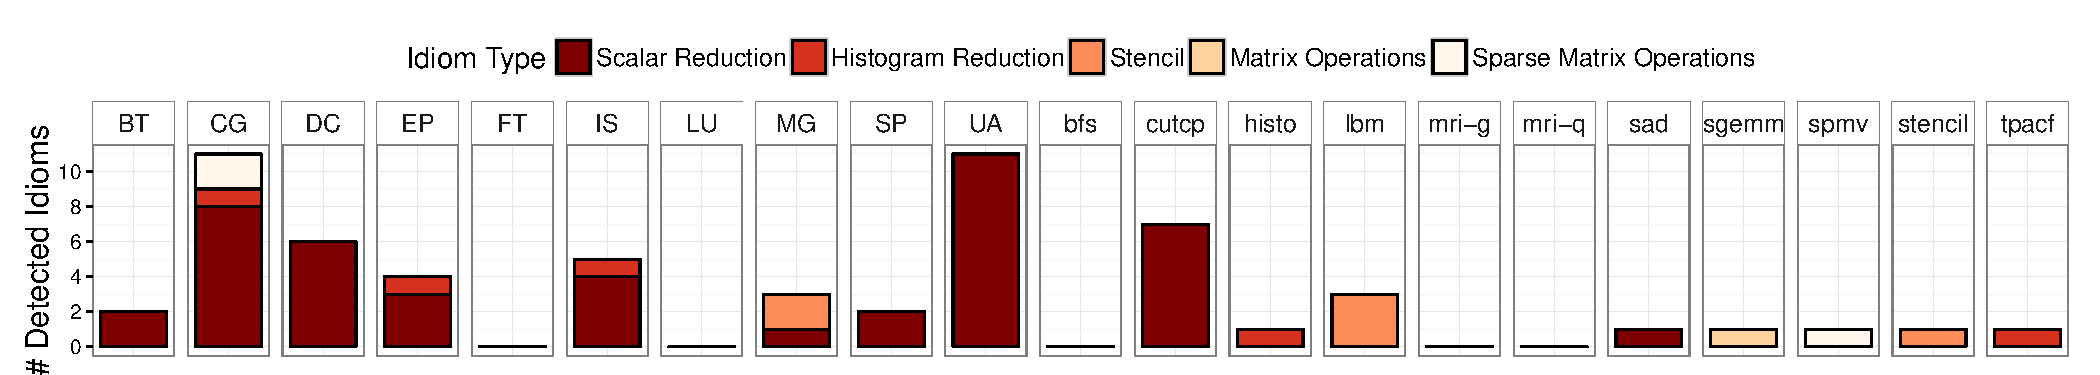
\includegraphics[width=\textwidth]{figures/asplos_detection.pdf}
  \caption{The different computational idioms found across the benchmark
           programs:
           Scalar reductions were the most common, with 10 out of 21 programs
           containing some.
           Other idioms were found in 1--5 programs each.
           Only five of the benchmarks contained no idiomatic code.}
  \label{detection-figure}
\end{figure}
\begin{figure}[p]
  \centering
  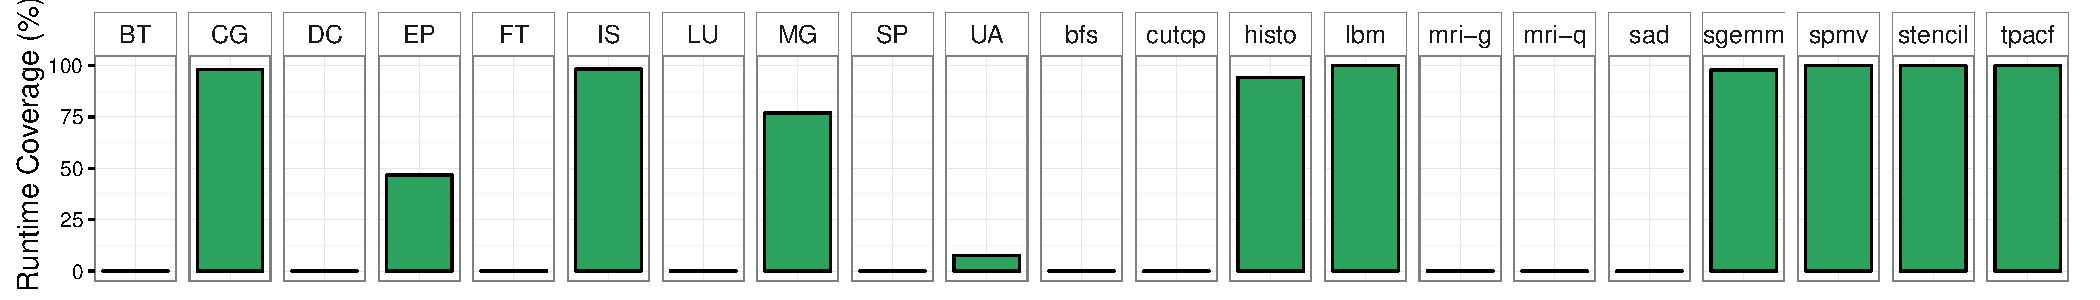
\includegraphics[width=\textwidth]{figures/asplos_coverage.pdf}
  \caption{Run time coverage: 10 of the 21 programs have idiomatic performance
           bottlenecks.\leftskip=0pt\rightskip=0pt}
  \label{coverage-figure}
  \vspace{0.5em}
\end{figure}

\begin{table}[p]
\centering
  \begin{tabular}{lP{2.16cm}P{2.16cm}P{2.16cm}P{2.163cm}P{2.163cm}}
  \toprule
  \hspace{1.18cm} & Scalar\newline{}Reduction & Histogram\newline{}Reduction & Stencil & Matrix~Op. & Sparse\newline{}Matrix~Op.\\
  \midrule
  Polly &  3  &  --- &   5  &   1  & --- \\
  ICC   &  28 &  --- &  --- &  --- & --- \\
  IDL   &  45 &   5  &   6  &   1  &  3  \\
  \bottomrule
\end{tabular}
\caption{Idioms detected by IDL, ICC, Polly}
\label{tab:detection}
\end{table}

\begin{table}[p]
\centering
\begin{tabular}{lcccccccccccc}
  \toprule
  & \hspace{0.17mm}BT\hspace{0.17mm}
  & \hspace{0.17mm}CG\hspace{0.17mm}
  & \hspace{0.17mm}DC\hspace{0.17mm}
  & \hspace{0.17mm}EP\hspace{0.17mm}
  & \hspace{0.17mm}FT\hspace{0.17mm}
  & \hspace{0.17mm}IS\hspace{0.17mm}
  & \hspace{0.17mm}LU\hspace{0.17mm}
  & \hspace{0.17mm}MG\hspace{0.17mm}
  & \hspace{0.17mm}SP\hspace{0.17mm}
  & \hspace{0.17mm}UA\hspace{0.17mm}
  & \hspace{0.17mm}bfs\hspace{0.17mm}
  & \hspace{0.17mm}cutcp\hspace{0.17mm} \\
  \midrule
without IDL    & 1.9 & 0.5 & 1.0 & 0.3 & 0.6 & 0.3 & 1.9 & 0.8 & 1.6 & 2.7 & 0.4 & 0.4 \\[0.25em]
with IDL       & 4.0 & 0.8 & 1.6 & 0.6 & 1.2 & 0.5 & 3.9 & 4.5 & 3.2 & 7.3 & 0.5 & 0.6 \\[0.75em]
overhead in \% & 116 &  77 &  57 &  77 &  93 &  62 & 103 & 484 &  97 & 169 &  30 &  65 \\
  \bottomrule
\end{tabular}
\begin{tabular}{lccccccccc}
  \toprule
  & \hspace{0.44mm}histo\hspace{0.44mm}
  & \hspace{0.44mm}lbm\hspace{0.44mm}
  & \hspace{0.44mm}mri-g\hspace{0.44mm}
  & \hspace{0.44mm}mri-q\hspace{0.44mm}
  & \hspace{0.44mm}sad\hspace{0.44mm}
  & \hspace{0.44mm}sgemm\hspace{0.44mm}
  & \hspace{0.44mm}spmv\hspace{0.44mm}
  & \hspace{0.44mm}stencil\hspace{0.44mm}
  & \hspace{0.44mm}tpacf\hspace{0.44mm} \\
  \midrule
without IDL    & 0.2 & 0.3 & 0.2 & 0.2 & 0.4 & 0.6 & 0.3 & 0.2 & 0.2 \\[0.25em]
with IDL       & 0.2 & 0.6 & 0.4 & 0.3 & 0.6 & 0.7 & 0.7 & 0.2 & 0.4 \\[0.75em]
overhead in \% &  35 &  87 & 100 &  52 &  58 &  24 & 115 &  36 &  54 \\
  \bottomrule
\end{tabular}
\caption{Compile time cost in seconds}
\label{tab:compiletimecost}
\end{table}

\subsection{Runtime Coverage}

    To determine if the detected idioms were impactful, \Cref{coverage-figure}
    shows the percentage of run time spent in the detected computational idiom
    for each benchmark program.
    This data shows that either the detected idioms have a low runtime
    contribution or they dominate almost the entire execution.
    \emph{EP} is the only exception with about 50\% run time coverage.
    Heterogeneous acceleration was evaluated on the ten programs that spend a
    significant amount of time in the detected idioms.
    Only these can reasonably expect a performance gain.

\subsection{Performance Results}

\paragraph*{Speedup over Sequential}

    \Cref{fig:speedup-figure} shows the end-to-end speedup obtained by
    accelerating idioms via heterogeneous APIs on a CPU, an integrated GPU,
    and an external GPU.
    All of the results include data transfer overhead to and from the GPUs,
    where required.
    This overhead is intrinsic to the external GPU, which operate on distinct
    physical memory.
    The integrated GPU, on the other hand, only incurred this cost when APIs
    enforced additional data copies.
    Each bar shows the best-performing API for the given platform;
    \Cref{tab:detailed-results} provides detailed results also for the other
    API backends.

\begin{figure}[t]
  \centering
  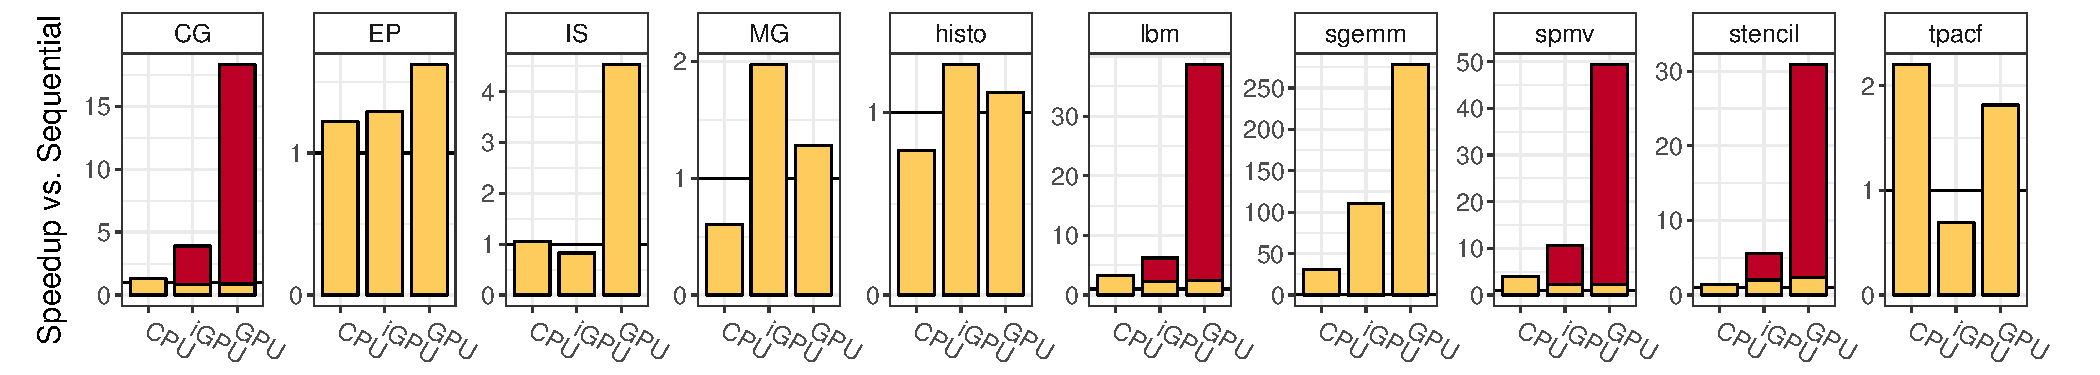
\includegraphics[width=\textwidth]{figures/asplos_speedup.pdf}
  \caption{Speedup over sequential:
           Results for the best-performing backend on each platform are shown.
           The red bars indicate a manual modification for minimising redundant
           data transfers.}
  \label{fig:speedup-figure}
  \vspace{1.5em}
  \centering
  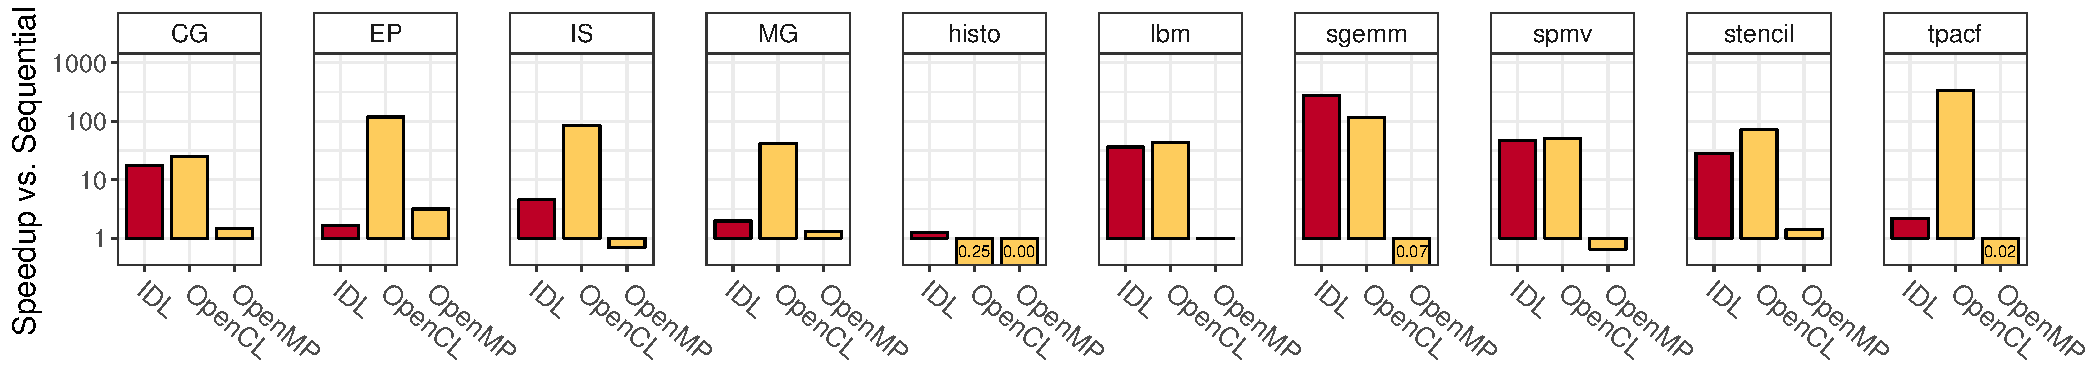
\includegraphics[width=\textwidth]{figures/asplos_comparison.pdf}
  \caption{IDL versus manual expert parallelisation:
           Speedup over the sequential baseline was measured for IDL
           (selecting best performing backend; red bars) and the
           handwritten reference OpenCL and OpenMP implementations
           (provided by the benchmark developers; yellow bars).}
  \label{fig:speedup-figure-2}
  \vspace{0.5em}
\end{figure}

    Moderate speedups were obtained for five of the benchmarks, from
    1.26$\times$ for ``\emph{histo}'' up to 4.5$\times$ for `\emph{IS}''.
    Besides ``\emph{MG}'', all of these benchmarks have a scalar or histogram
    reduction as their performance bottleneck.
    Interestingly, we can see that for different benchmarks, different hardware
    is beneficial.
    For ``\emph{tpcaf}'', the CPU is the best platform, beating the GPU,
    for which the data transfer time dominates;
    for ``\emph{MG}'' and ``\emph{histo}'', the integrated GPU strikes the right
    balance between computational power and avoiding data movement to the
    external GPU;
    and for ``\emph{EP}'' and ``\emph{IS}'', the data transfer to the GPU is
    amortised by its superior raw performance.
    The results emphasise the significance of flexible heterogeneous
    code generation.
    Committing to any one of the three hardware platforms in the source code
    would have necessarily resulted in less-than-optimal performance for at
    least some of the programs.

    For five of the benchmarks, IDL enabled significantly higher performance
    gains, from 17$\times$ for ``\emph{CG}'' and up to over 275$\times$ for
    ``\emph{sgemm}''.
    These benchmarks are computationally expensive, and the external GPU is
    always the fastest architecture by a considerable margin.

\begin{landscape}
\newlength{\txtwd}
\newcommand{\msb}[1]{\settowidth{\txtwd}{#1}{\tiny\ttfamily\bfseries \hfill #1}}
\newcommand{\ms}[1]{\settowidth{\txtwd}{#1}{\tiny\ttfamily \hfill #1}}
\addtolength{\tabcolsep}{-0.64mm}
\begin{table}[p]
  \centering
  \small
  \begin{tabular}{|l||cccccc|ccccc|cccc|}
  \hline
  & \multicolumn{6}{c|}{\bfseries\large CPU} & \multicolumn{5}{c|}{\bfseries\large iGPU} & \multicolumn{4}{c|}{\bfseries\large GPU} \\
  & MKL & libSPMV & Halide & clBLAS & CLBlast & Lift & clSPARSE & libSPMV & clBLAS & CLBlast & Lift & cuSPARSE & libSPMV & cuBLAS & Lift \\
  \hline
  \hline
   CG      & \msb{1504.21} & --- & --- & --- & --- & --- & \msb{644.02} & --- & --- & --- & --- &  \msb{113.51} & --- & --- & --- \\[3mm]
   EP      & --- & --- & --- & --- & --- &  \msb{32762.50}  & --- & --- & --- & --- & \msb{30983.40}  & --- & --- & --- & \msb{24680.70} \\[3mm]
   IS      & --- & --- & \msb{426.95} & ---  & --- & \ms{1765.61}  &  --- & --- & --- & --- & \msb{547.28}  & --- & --- & --- & \msb{99.95} \\[3mm]
   MG      & --- & --- & --- & --- & --- &  \msb{4699.63}  & --- & --- & --- & --- & \msb{1439.58}  & --- & --- & --- & \msb{2211.56} \\[3mm]
   histo   & --- & --- & --- & --- & --- &  \msb{27.42}  & --- & --- & --- & --- & \msb{17.20}  & --- & --- & --- & \msb{19.54} \\[3mm]
   lbm     & --- & --- & --- & --- & --- &  \msb{6457.93}  & --- & --- & --- & --- & \msb{5335.09}  & --- & --- & --- & \msb{590.60} \\[3mm]
   sgemm   & \msb{53.50} & --- & --- & \ms{1661.75} & \ms{660.44} & \ms{1339.15}  & --- & --- & \msb{14.73} & \ms{19.03} & \ms{15.04}  & --- & --- & \msb{5.99} & \ms{7.87} \\[3mm]
   spmv    & --- & \msb{218.17} & --- & --- & --- & --- & --- &\msb{102.233} & --- & --- & --- & --- &\msb{18.437} & --- &  ---\\[3mm]
   stencil & --- & ---& \msb{5760.81} & --- & --- & \ms{21951.80}  & --- & ---& --- & --- & \msb{2261.48} & --- & ---& --- & \msb{279.38} \\[3mm]
   tpacf   & --- & ---& --- & --- & --- & \msb{19276.40}  & --- & ---& --- & --- & \msb{61111.90} & --- & ---& --- & \msb{23358.20} \\
  \hline
\end{tabular}
\caption{Detailed performance results for each heterogeneous backend interface:
         The run time of each benchmark program was measured in milliseconds for
         every compatible combination on each of the three platforms.
         The fastest implementations for per benchmark and target hardware are
         highlighted in {\bf bold}.}
\label{tab:detailed-results}
\end{table}
\end{landscape}

    The red highlighting in \Cref{fig:speedup-figure} indicates an important
    runtime optimisation:
    Redundant data transfers for the iterative ``\emph{CG}'', ``\emph{lbm}'',
    ``\emph{spmv}'' and ``\emph{stencil}'' benchmarks were manually eliminated.
    All of these benchmarks execute computations inside a for-loop and do not
    require access to the data on the CPU between iterations.
    A straightforward lazy copying technique was manually applied by flagging
    memory objects to avoid redundant transfers, similar
    to work by \citet{jablin11automatic}.
    This runtime optimisation is crucial for achieving high performance on some
    of the benchmark programs.

\paragraph*{API performance comparison}

    \Cref{tab:detailed-results} shows a breakdown of the performance of each API
    on each program and platform.
    Not all APIs target all platforms, {\emph{e.g.} cuSPARSE only targets NVIDIA
    GPUs.
    The version of Halide that was used for this evaluation failed to generate
    valid GPU code for any of the benchmarks.
    Therefore, only the CPU platform was evaluated with Halide.
    The best-performing backend is highlighted in bold in the table entries.
    None of the previously existing backends supported SPMV-JDS, which was used
    by the ``\emph{spmv}'' benchmark.
    The libSPMV library was implemented as an ad-hoc solution to this,
    providing straightforward parallelisation of the idiom.

    On the multi-core CPU, Intel MKL gave the best linear algebra performance,
    outperforming the other libraries and Lift.
    Halide achieved good performance for the NPB ``\emph{IS}'' and Parboil
    ``\emph{stencil}'' benchmarks on the CPU, outperforming Lift due to its more
    advanced vectorisation capabilities.
    In the programs where scalar reductions dominate, Lift performed well.
    On the iGPU, clBLAS provides a better matrix-multiplication implementation
    than either CLBlast or Lift.
    On the external GPUs, library backends provided the best linear algebra
    implementations, while Lift performed well on stencils and reductions.

\paragraph*{Speedup vs Handwritten Parallel Implementations}

    \Cref{fig:speedup-figure-2} shows the performance of the IDL approach
    compared to handwritten reference OpenMP and OpenCL implementations.
    For some of the benchmarks, the parallel versions are significantly modified
    and use different algorithms beyond the reach of automation.
    For benchmarks where the parallel reference implementation does not make
    profound algorithmic changes (``\emph{CG}'', ``\emph{histo}'',
    ``\emph{lbm}'', ``\emph{sgemm}'', ``\emph{spmv}'', ``\emph{stencil}''),
    IDL enabled comparable -- or better -- performance.
    For four benchmarks (``\emph{EP}'', ``\emph{IS}'', ``\emph{MG}'',
   ``\emph{tpacf}'') it is beneficial to parallelise the entire application,
    which is beyond the scope of this work.

    The handwritten versions of ``\emph{sgemm}'' and ``\emph{stencil}' were
    outperformed by IDL.
    This was due to implementation flaws, a loop interchange already improved
    performance by almost 20$\times$.

\paragraph*{Summary}

    60 idioms were detected across the benchmark suites, and significant
    performance improvements were achieved by targeting different heterogeneous
    APIs for those benchmarks where idioms dominate execution time.

\section{Conclusions}

    The chapter developed a compiler-based approach that automatically detects
    a broad class of computational idioms that are supported by libraries or
    domain-specific languages targeting heterogeneous computing.
    The approach is based on the declarative Idiom Detection Language that
    identifies program subsets adhering to idiom specifications with a
    constraint solver.
    Once detected, the idiomatic loops were mechanically translated into API
    calls to external libraries or to code generated by DSL compilers.

    The approach was evaluated on the C/C++ programs from two well-known
    benchmark suites: NAS and Parboil.
    IDL detected more stencils, sparse matrix operations and generalised
    reduction and histogram computations than existing approaches, and it
    generated fast code.
